\documentclass[a4paper, 11pt]{ctexart}

% 页面设置
\usepackage{geometry}
\geometry{a4paper, left=2.5cm, right=2.5cm, top=2.5cm, bottom=2.5cm}

% 数学公式与符号
\usepackage{amsmath}
\usepackage{amssymb}

% 图片与代码
\usepackage{graphicx}
\graphicspath{{figures/}}
\usepackage{float}
\usepackage{listings}
\usepackage{xcolor}
\usepackage{booktabs}


\lstset{
    language=Matlab,
    basicstyle=\ttfamily\small,
    keywordstyle=\color{blue},
    commentstyle=\color{green!50!black},
    stringstyle=\color{purple},
    frame=single,
    breaklines=true,
    numbers=left,
    numberstyle=\tiny\color{gray}
}

\title{\textbf{基于 MATLAB 的 OFDM 数字通信系统仿真分析报告}}
\author{李嘉豪 \quad 3023234059}
\date{\today}

\begin{document}

\maketitle

\begin{abstract}
本报告围绕正交频分复用（OFDM）技术展开 MATLAB 仿真分析，共分三个部分。第一部分建立离散多径信道模型，分别改变第二径的时延位置、幅度、相位，并引入多径，研究信道参数对频率响应的影响。第二部分搭建基于 IFFT/FFT 的 OFDM 基带传输链路，在 AWGN 信道下对比 BPSK、QPSK 和 16-QAM 三种调制方式的误码性能。第三部分在系统中加入循环前缀（CP）与迫零频域均衡，在多径信道环境下验证其消除符号间干扰的有效性。仿真结果表明，OFDM 技术配合频域均衡能够有效应对频率选择性衰落，不同调制阶数在频谱效率与抗噪声性能之间存在明显折中。
\end{abstract}

\section{绪论}

\subsection{实验背景}
在无线通信系统中，由于传播环境中的反射、折射与散射，接收端信号通常是多条不同路径信号的叠加，即多径效应。多径传播会导致信号在时域上产生时延扩展，进而在频域上引起频率选择性衰落。当系统传输带宽大于信道的相干带宽时，信号会发生严重的符号间干扰 (ISI)。正交频分复用 (OFDM) 技术通过将宽带信道划分为多个正交的窄带子信道，能够有效抵抗频率选择性衰落。

\subsection{实验目的}
本实验主要分为三个部分：
\begin{enumerate}
    \item HOMEWORK I. 建立离散多径信道模型，分析信道参数（时延、幅度、相位）对频率响应特性的影响。
    \item HOMEWORK II. 搭建基于 IFFT/FFT 的基础 OFDM 通信链路，验证其在 AWGN 信道下的性能。
    \item HOMEWORK III. 在 OFDM 系统中引入循环前缀 (CP) 与零迫频域均衡，验证其在多径信道下消除 ISI 的有效性。
\end{enumerate}

\section{多径信道特性研究}

\subsection{时延扩展的理论推导}
建立双径离散时间信道模型。假设第一条路径为主径，增益为 1，无延迟；第二条路径为反射径，相对增益为 $\alpha$，相对延迟为 $\tau$ 个采样周期。该信道的离散时间冲激响应 $h(n)$ 表示为：
\begin{equation}
    h(n) = \delta(n) + \alpha \delta(n - \tau)
\end{equation}

对其进行离散时间傅里叶变换 (DTFT)，可得频率响应 $H(e^{j\omega})$：
\begin{equation}
    H(e^{j\omega}) = 1 + \alpha e^{-j\omega\tau}
\end{equation}

对应的幅度频率响应 $|H(e^{j\omega})|$ 为：
\begin{equation}
    |H(e^{j\omega})| = \sqrt{(1 + \alpha\cos(\omega\tau))^2 + (-\alpha\sin(\omega\tau))^2} = \sqrt{1 + \alpha^2 + 2\alpha\cos(\omega\tau)}
\end{equation}
由式 (3) 可知，信道的幅度响应在频域上呈现余弦周期性振荡，这反映了多径叠加导致的频率选择性衰落特性。


%---------------------------------------------------------------------------------------------------------------------------------
\subsection{改变第二径位置对频率响应的影响}

\subsubsection{频域特性仿真与代码实现}
为了定量分析时延扩展对信道相干带宽的影响，本节通过 MATLAB 仿真，保持第二径的幅度 $\alpha = 0.5$ 恒定，分别设置第二径延迟 $\tau = 3, 7, 15$（单位：采样周期），计算并绘制信道的幅度与相位频率响应。

\begin{lstlisting}[caption={不同延迟梯度下的信道频率响应仿真代码}]
clear; clc; close all;

N_fft = 1024; 
f = linspace(0, 1, N_fft); 
delays = [3, 7, 15]; 
colors = {'#0072BD', '#D95319', '#EDB120'}; 

figure('Position', [100, 100, 800, 600]);

for i = 1:length(delays)
    tau = delays(i);
    h = zeros(1, tau + 1);
    h(1) = 1;                   
    h(tau + 1) = 0.5;           
    
    H = fft(h, N_fft);          
    H_mag = abs(H);             
    H_phase = unwrap(angle(H)); 
    
    subplot(2, 1, 1); hold on;
    plot(f, H_mag, 'Color', colors{i}, 'LineWidth', 1.5, ...
         'DisplayName', ['Delay \tau = ', num2str(tau)]);
         
    subplot(2, 1, 2); hold on;
    plot(f, H_phase, 'Color', colors{i}, 'LineWidth', 1.5, ...
         'DisplayName', ['Delay \tau = ', num2str(tau)]);
end

subplot(2, 1, 1);
grid on; xlabel('归一化频率'); ylabel('幅度 |H(f)|');
title('不同时延扩展下的信道幅度响应对比');
legend('Location', 'best');

subplot(2, 1, 2);
grid on; xlabel('归一化频率'); ylabel('相位 (rad)');
title('不同时延扩展下的信道相位响应对比');
legend('Location', 'best');
\end{lstlisting}

\subsubsection{频域响应分析}
% 插入运行上述代码得到的双子图
\begin{figure}[H]
    \centering
    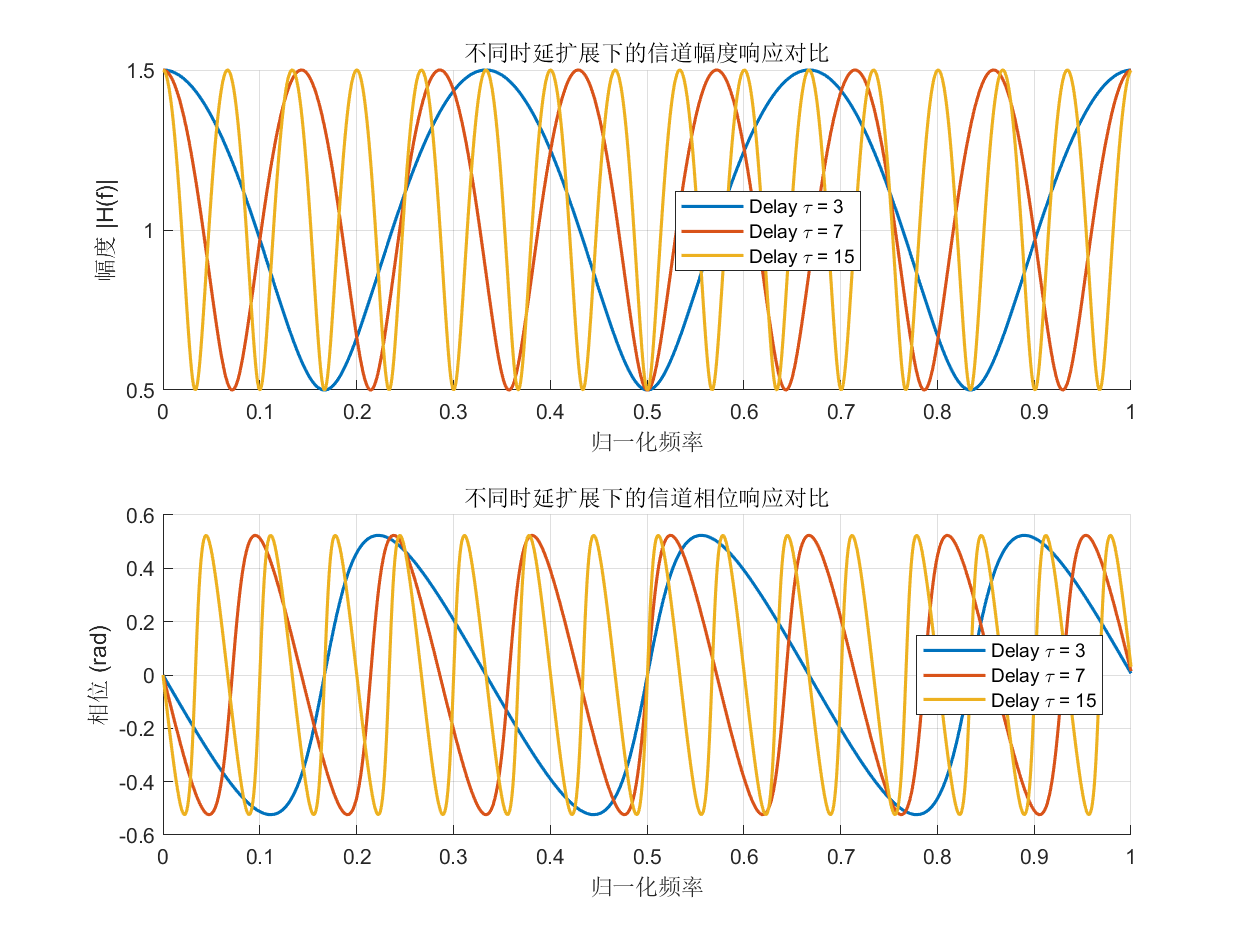
\includegraphics[width=0.9\textwidth]{hw1_delay_mag_phase.png}
    \caption{第二径延迟对信道幅度与相位响应的影响}
\end{figure}

\subsubsection{结果分析与描述}
从图中可以看到，随着第二径延迟 $\tau$ 从 3 增大到 15，幅度频率响应的振荡周期明显缩短，频域内的衰落波谷变得更加密集，同时相位响应的非线性也相应增强。根据幅度公式 $|H(e^{j\omega})| = \sqrt{1.25 + \cos(\omega\tau)}$，时域延迟 $\tau$ 相当于频域余弦波动的角频率，$\tau$ 越大，直射波与反射波之间的相位差随频率变化得越快，因此在更窄的频带内就完成了一个完整的衰落周期。这一结果直接说明了信道的最大时延扩展 $\tau_m$ 与相干带宽 $B_c$ 之间的反比关系：时延越大，相干带宽越小，频率选择性衰落越严重。
%---------------------------------------------------------------------------------------------------------------------------------
\subsection{改变第二径幅度对频率响应的影响}

\subsubsection{幅频响应的极值分析}
在多径信道中，频率选择性衰落的深度受各路径相对增益的影响。由幅度频率响应的理论公式：
\begin{equation}
    |H(e^{j\omega})| = \sqrt{1 + \alpha^2 + 2\alpha \cos(\omega\tau)}
\end{equation}
可知，当 $\cos(\omega\tau) = 1$ 时，信道取得最大增益 $|H|_{max} = 1 + \alpha$；当 $\cos(\omega\tau) = -1$ 时，信道出现最深衰落，其极小值为 $|H|_{min} = |1 - \alpha|$。

这表明，衰落深度由主径与反射径的幅度差 $|1-\alpha|$ 决定。当反射径幅度 $\alpha$ 趋近于主径幅度 1 时，衰落波谷将趋近于零，形成深衰落（Deep Fading）。

\subsubsection{频域特性仿真与代码实现}
为验证幅度 $\alpha$ 对衰落深度的影响，本仿真固定第二径延迟 $\tau = 5$ 采样周期，分别设置第二径幅度 $\alpha = 0.2, 0.5, 0.8, 1.0$ 进行对比分析。

\begin{lstlisting}[caption={不同路径幅度下的信道频率响应仿真代码}]
clear; clc; close all;

N_fft = 1024; 
f = linspace(0, 1, N_fft);
tau = 5; 
alphas = [0.2, 0.5, 0.8, 1.0]; 
colors = {'#77AC30', '#0072BD', '#D95319', '#A2142F'};

figure('Position', [100, 100, 800, 400]);
hold on;

for i = 1:length(alphas)
    a = alphas(i);
    h = zeros(1, tau + 1);
    h(1) = 1;
    h(tau + 1) = a;
    
    H_mag = abs(fft(h, N_fft));
    plot(f, H_mag, 'Color', colors{i}, 'LineWidth', 1.5, ...
         'DisplayName', ['Amplitude \alpha = ', num2str(a)]);
end

yline(0, '--k', 'HandleVisibility', 'off'); 
grid on; xlabel('归一化频率'); ylabel('幅度 |H(f)|');
title('不同反射径幅度对信道衰落深度的影响');
legend('Location', 'northeast');
\end{lstlisting}

\subsubsection{结果分析}
% 插入运行上述代码得到的图片
\begin{figure}[H]
    \centering
     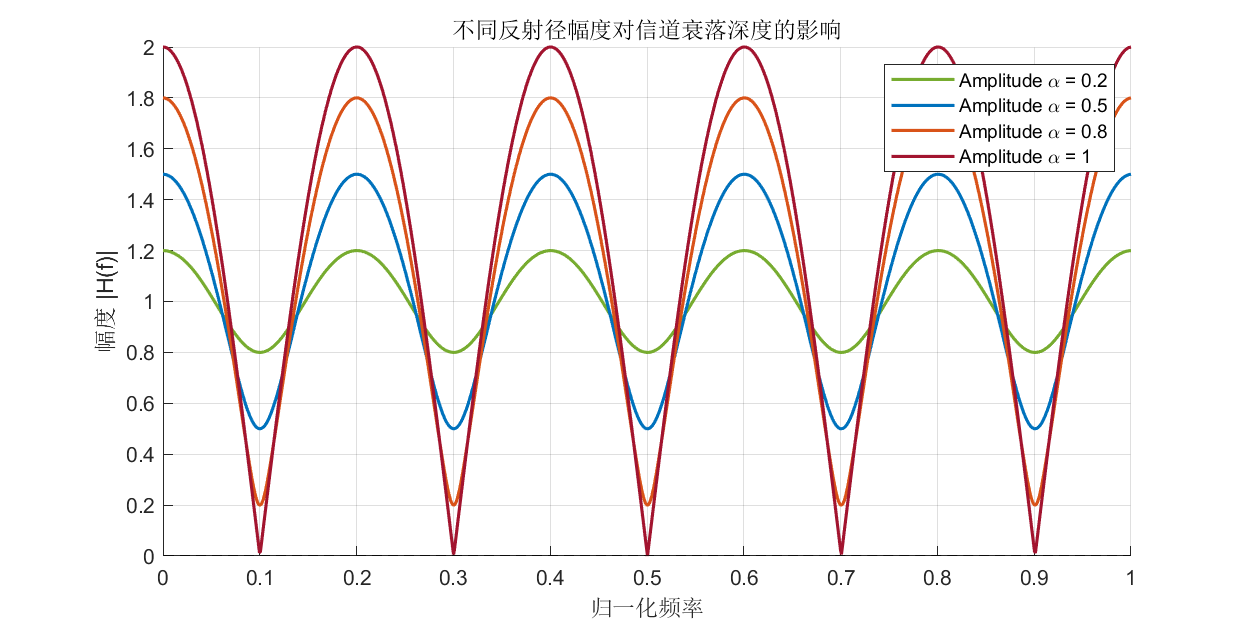
\includegraphics[width=0.8\textwidth]{hw1_amplitude.png}
    \caption{第二径幅度对频率选择性衰落深度的影响}
\end{figure}

\subsubsection{结果分析与描述}
从图中可以看出，随着 $\alpha$ 从 0.2 增大到 1.0，频域波形的振荡幅度逐渐增大。波峰抬升至 $1+\alpha$，波谷下沉至 $|1-\alpha|$。当 $\alpha = 1.0$ 时，反射径与主径幅度相等，频率响应的波谷刚好到达零点，形成完全衰落。这是因为在该频点处两路信号恰好反相，幅度相等导致完全相消。这一结果说明衰落深度取决于主径与反射径的幅度比：两者越接近，衰落越深。对于宽带传输而言，这种深衰落意味着某些子载波的信号会被严重衰减，需要通过频域均衡和信道编码来恢复。
%---------------------------------------------------------------------------------------------------------------------------------
\subsection{改变两径相位对频率响应的影响}

\subsubsection{相位偏移的频域等效}
当反射径相对于主径存在额外的相位偏差 $\theta$ 时，双径信道的离散时间冲激响应表示为：
\begin{equation}
    h(n) = \delta(n) + \alpha e^{j\theta} \delta(n - \tau)
\end{equation}

对其进行离散时间傅里叶变换，可得信道的频率响应：
\begin{equation}
    H(e^{j\omega}) = 1 + \alpha e^{j\theta} e^{-j\omega\tau} = 1 + \alpha e^{-j(\omega\tau - \theta)}
\end{equation}

计算其幅度频率响应的模值：
\begin{equation}
    |H(e^{j\omega})| = \sqrt{1 + \alpha^2 + 2\alpha \cos(\omega\tau - \theta)}
\end{equation}
式 (7) 表明，相位差 $\theta$ 在频域余弦函数中表现为一个常数相位偏移项。

\subsubsection{频域特性仿真与代码实现}
固定第二径延迟 $\tau = 3$ 与幅度 $\alpha = 0.5$。分别模拟同相（$\theta = 0^\circ$）与反相（$\theta = 180^\circ$）两种信道状态，计算其幅度频率响应。

\begin{lstlisting}[caption={不同反射径相位下的信道频率响应仿真代码}]
clear; clc; close all;

N_fft = 1024; 
f = linspace(0, 1, N_fft); 
tau = 3; 

h1 = zeros(1, tau + 1);
h1(1) = 1;
h1(tau + 1) = 0.5; % 相位差 0 度

h2 = zeros(1, tau + 1);
h2(1) = 1;
h2(tau + 1) = -0.5; % 相位差 180 度 (相当于乘以 -1)

H1_mag = abs(fft(h1, N_fft));
H2_mag = abs(fft(h2, N_fft));

figure('Position', [100, 100, 800, 400]);
hold on;
plot(f, H1_mag, 'Color', '#0072BD', 'LineWidth', 1.5, 'DisplayName', '\theta = 0^\circ');
plot(f, H2_mag, 'Color', '#D95319', 'LineStyle', '--', 'LineWidth', 1.5, 'DisplayName', '\theta = 180^\circ');

grid on; xlabel('归一化频率'); ylabel('幅度 |H(f)|');
title('改变第二径相位对信道幅度响应的影响');
legend('Location', 'northeast');
\end{lstlisting}

\subsubsection{极值频点计算与结果分析}
% 插入运行上述代码得到的图片
\begin{figure}[H]
    \centering
    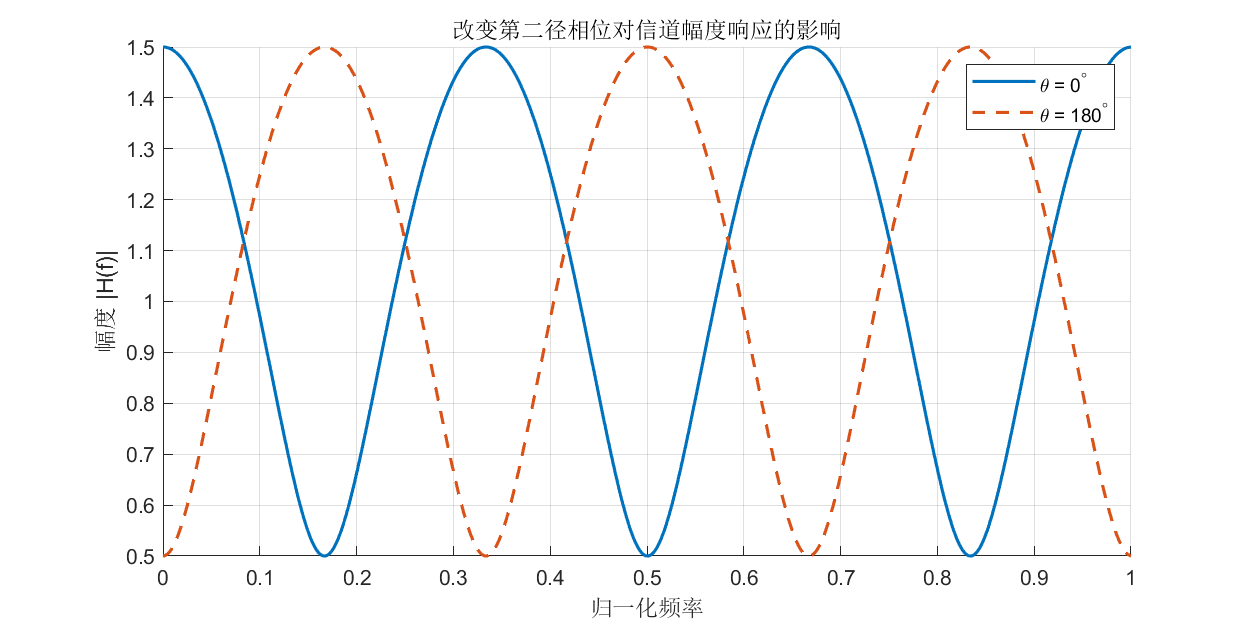
\includegraphics[width=0.8\textwidth]{hw1_phase.png} 
    \caption{第二径相位反转对幅度频率响应的平移作用}
\end{figure}

为了定量分析相位偏移 $\theta$ 对频域曲线的具体影响，对衰落波谷（极小值）所在的频点进行数学求解。设归一化数字频率为 $f$，则 $\omega = 2\pi f$。由极值条件可知，当 $\cos(2\pi f \tau - \theta) = -1$ 时，信道出现最深衰落。

代入仿真参数 $\alpha = 0.5, \tau = 3$：

\textbf{情况一：同相信道 ($\theta = 0$)}
极值条件为 $\cos(6\pi f) = -1$，解得：
\begin{equation*}
    6\pi f = (2k + 1)\pi \quad (k = 0, 1, 2, \dots)
\end{equation*}
在 $f \in [0, 1]$ 范围内，衰落波谷出现的频率点为：
\begin{equation*}
    f_1 = \frac{1}{6} \approx 0.1667, \quad f_2 = \frac{1}{2} = 0.5, \quad f_3 = \frac{5}{6} \approx 0.8333
\end{equation*}

\textbf{情况二：反相信道 ($\theta = \pi$)}
极值条件为 $\cos(6\pi f - \pi) = -1$，解得：
\begin{equation*}
    6\pi f - \pi = (2k + 1)\pi \implies 6\pi f = 2(k + 1)\pi \quad (k = 0, 1, 2, \dots)
\end{equation*}
在 $f \in [0, 1]$ 范围内，衰落波谷出现的频率点为：
\begin{equation*}
    f'_1 = \frac{1}{3} \approx 0.3333, \quad f'_2 = \frac{2}{3} \approx 0.6667, \quad f'_3 = 1.0
\end{equation*}

计算结果与仿真图吻合。对比两种情况的波谷频点，引入 $\theta = 180^\circ$ 的相位差后，幅度响应曲线在频率轴上整体平移了 $\Delta f = 1/6$。但相邻波谷之间的频率间隔保持不变，均为 $1/3$，波峰和波谷的极值大小也没有改变。这说明多径分量的相位差只会影响频率选择性衰落发生在哪些频点上，不会改变衰落的周期和深度。
%---------------------------------------------------------------------------------------------------------------------------------

\subsection{引入复杂多径环境对频率响应的影响}

\subsubsection{多径叠加的泛化表达}
在真实的城市或室内无线通信环境中，接收信号通常是大量反射径、散射径的叠加。此时，离散时间冲激响应扩展为 $L$ 径模型：
\begin{equation}
    h(n) = \sum_{i=0}^{L-1} \alpha_i \delta(n - \tau_i)
\end{equation}
对其进行离散时间傅里叶变换，可得信道的频率响应：
\begin{equation}
    H(e^{j\omega}) = \sum_{i=0}^{L-1} \alpha_i e^{-j\omega\tau_i}
\end{equation}
其幅度频率响应 $|H(e^{j\omega})|$ 包含了多个具有不同周期和相位的复指数项的叠加。与双径模型中规则的余弦振荡不同，复杂多径环境下的幅度响应曲线将呈现出不规则的起伏特性。

\subsubsection{频域特性仿真与代码实现}
本仿真对比了标准双径信道与复杂五径信道的频率响应。
\begin{itemize}
    \item 双径模型：$h_2 = [1, 0, 0, 0.5]$
    \item 五径模型：$h_5 = [1, 0, 0.4, 0, -0.3, 0.2, 0, 0.1]$
\end{itemize}

\begin{lstlisting}[caption={复杂多径环境下的信道频率响应仿真代码}]
clear; clc; close all;

N_fft = 1024; 
f = linspace(0, 1, N_fft); 

% 构建双径与五径信道模型
h_2path = [1, 0, 0, 0.5];
h_5path = [1, 0, 0.4, 0, -0.3, 0.2, 0, 0.1];

% 计算离散傅里叶变换
H2_mag = abs(fft(h_2path, N_fft));
H5_mag = abs(fft(h_5path, N_fft));

figure('Position', [100, 100, 700, 400]);
hold on;
plot(f, H2_mag, 'Color', '#0072BD', 'LineWidth', 1.5, 'DisplayName', '双径信道 (2径)');
plot(f, H5_mag, 'Color', '#D95319', 'LineStyle', '-', 'LineWidth', 1.5, 'DisplayName', '复杂信道 (5径)');

grid on; xlabel('归一化频率'); ylabel('幅度 |H(f)|');
title('复杂多径环境下的信道幅度响应对比');
legend('Location', 'northeast');
\end{lstlisting}

\subsubsection{结果分析}
% 插入图片占位符
\begin{figure}[H]
    \centering
    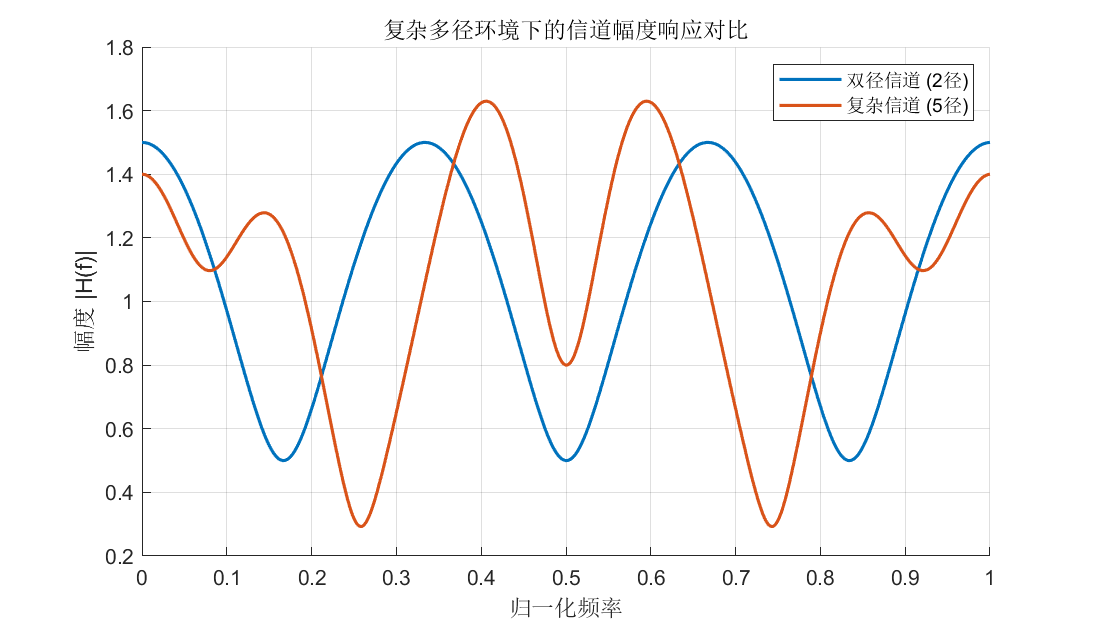
\includegraphics[width=0.8\textwidth]{hw1_multipath.png} 

    \caption{双径信道与复杂五径信道的幅度频率响应对比}
\end{figure}

\subsubsection{结果分析与描述}
从图中可以看到，将双径模型扩展为包含五条径的复杂信道后，幅度频率响应曲线由规则的余弦振荡变为不规则的起伏。这是因为系统频率响应从单一频率的余弦干涉，变为了多个不同频率、不同相位、不同权重的复指数项的叠加。多个反射分量的随机组合使得深衰落频点的分布失去了简单的周期规律。这种不规则的衰落特征更接近实际的无线信道环境，也说明了 OFDM 技术的实际价值：通过将宽带信道划分为多个窄带子载波，系统可以独立应对每个子载波上的衰落。


%---------------------------------------------------------------------------------------------------------------------------------
\section{基于 IFFT/FFT 的多调制 OFDM 系统仿真}

\subsection{本章引言}
第一章的分析表明，多径信道存在频率选择性衰落。如果在这样的信道中直接传输高速单载波信号，会导致严重的符号间干扰。OFDM 技术通过将宽带信道划分为 $N$ 个正交的窄带子载波，使每个子载波的带宽远小于信道的相干带宽，从而将频率选择性衰落转化为多个平坦衰落。本章构建基于 IFFT/FFT 的 OFDM 基带传输链路，在 AWGN 信道下对比 BPSK、QPSK 与 16-QAM 三种调制方式的传输性能。

\subsection{系统基带传输数学推导}
本节依据系统原理框图，对信号在链路中的演进过程进行数学建模。

\subsubsection{1. 信号调制 (Mod)}
系统接收二进制信源，将其映射为复平面上的离散物理符号 $X(k)$。本系统支持 $M \in \{2, 4, 16\}$ 阶调制，为保证后续抗噪性能对比的公平性，所有调制模式均施加平均功率归一化约束：
\begin{equation}
    E\left[|X(k)|^2\right] = 1, \quad k = 0, 1, \dots, N-1
\end{equation}

\subsubsection{2. IFFT 变换 ($s(n)$ 节点)}
串并转换后的频域符号 $X(k)$ 经 $N$ 点离散傅里叶反变换 (IFFT)，调制至各子载波上，合成为时域基带序列 $s(n)$：
\begin{equation}
    s(n) = \frac{1}{\sqrt{N}} \sum_{k=0}^{N-1} X(k) e^{j \frac{2\pi}{N} kn}, \quad n = 0, 1, \dots, N-1
\end{equation}
需指出，时域信号 $s(n)$ 由多个具有独立初相的正交正弦波叠加而成，当多数子载波同相叠加时会产生极高的瞬时峰值，导致系统出现高基带峰均功率比 (PAPR) 的物理现象。此外，公式采用 $1/\sqrt{N}$ 归一化以维持 IFFT 变换前后的能量守恒。

\subsubsection{3. AWGN 信道 ($r(n)$ 节点)}
在理想加性高斯白噪声 (AWGN) 信道模型下，时域信号叠加均值为零、方差为 $\sigma^2$ 的复高斯白噪声 $w(n)$：
\begin{equation}
    r(n) = s(n) + w(n)
\end{equation}

\subsubsection{4. FFT 变换 ($Y(k)$ 节点)}
接收端对 $r(n)$ 执行 $N$ 点离散傅里叶变换 (FFT)，利用复正弦基底的数学正交性实现各子载波的无损分离，解调出频域符号 $Y(k)$：
\begin{equation}
    Y(k) = \frac{1}{\sqrt{N}} \sum_{n=0}^{N-1} r(n) e^{-j \frac{2\pi}{N} kn} = X(k) + W(k)
\end{equation}
其中 $W(k)$ 为时域噪声经 FFT 映射后的频域复噪声分量。分离后的并行数据随后执行并串转换。

\subsubsection{5. 信号解调 (Demod)}
接收端获取串行 $Y(k)$ 后，依据最小欧氏距离原则（最大似然判决）在标准星座集 $\mathcal{C}$ 中进行判决，并逆向映射回二进制数据：
\begin{equation}
    \hat{X}(k) = \arg \min_{X_i \in \mathcal{C}} |Y(k) - X_i|^2
\end{equation}

\subsection{仿真环境与全局控制架构}
基于上述推演，在 MATLAB 环境中完成系统全局参数的初始化配置。该底层架构通过控制开关实现多调制阶数的遍历测试，为后续链路分级验证提供统一的信源。

\begin{lstlisting}[caption={系统全局变量初始化与信源生成代码}]
clear; clc; close all;

% --- 系统全局参数 ---
N_fft = 64;          % IFFT/FFT 点数
N_syms = 50000;      % OFDM 符号数
SNR_dB = 15;         % 单点演示信噪比

% 三种调制模式
mod_types = {'BPSK', 'QPSK', '16QAM'};
M_values  = [2, 4, 16];

% 二进制信源
numBits = N_fft * N_syms * log2(M);
tx_bits = randi([0 1], numBits, 1);
\end{lstlisting}


\subsubsection{环节一：信号调制结果与分析}

本环节的核心任务是完成数字基带信号的初始映射，将随机二进制比特流转化为频域复数符号序列。

\begin{lstlisting}[caption={环节一：发射端多阶信号调制核心代码}]
sim_data = struct();

for i = 1:length(mod_types)
    M = M_values(i);

    if M == 2
        X_k_serial = pskmod(tx_bits, M);
    else
        X_k_serial = qammod(tx_bits, M, ...
            'InputType', 'bit', 'UnitAveragePower', true);
    end

    sim_data(i).X_k_serial = X_k_serial;
end
\end{lstlisting}

\begin{figure}[H]
    \centering
    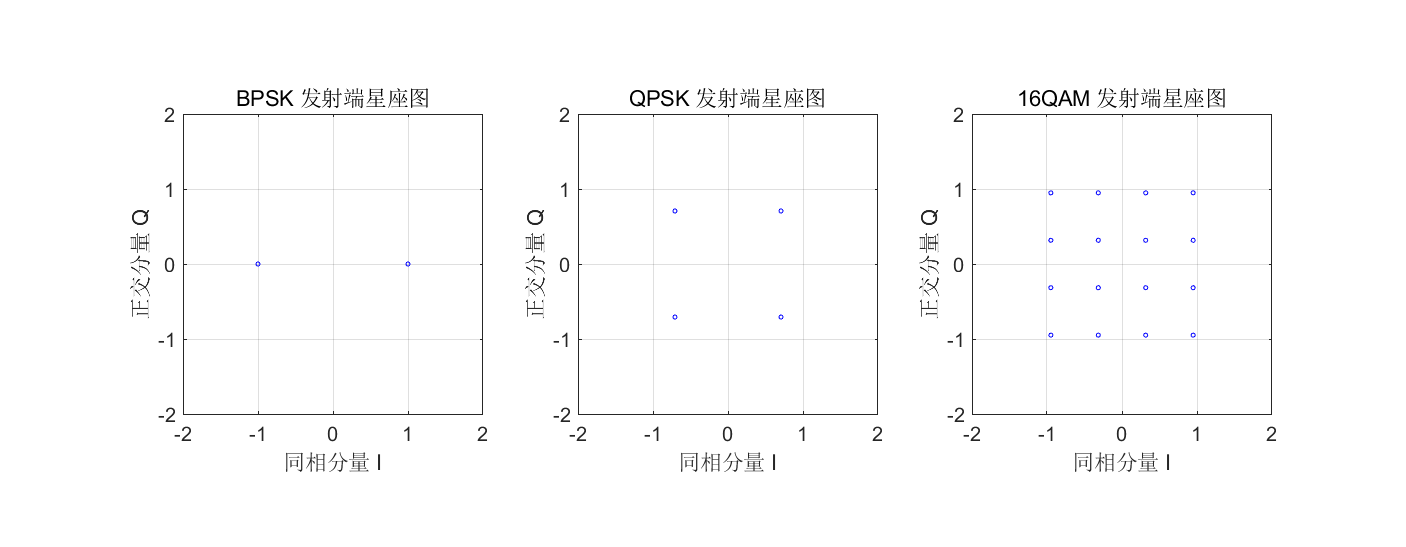
\includegraphics[width=1.0\textwidth]{hw2_step1_mod.png}
    \caption{发射端信号调制后的复平面星座图特征对比}
    \label{fig:step1_mod}
\end{figure}

结合上述代码与图 \ref{fig:step1_mod}，对环节一的结果进行分析：

从星座图来看，三种调制模式呈现出不同的分布特征。BPSK 只有两个符号点，分布在实轴上；QPSK 有四个符号点，对称分布在四个象限；16-QAM 有 16 个符号点，呈矩形网格排列。调制阶数越高，单个符号承载的比特数越多，但星座点之间的距离也越小，抗噪声能力相应减弱。

从功率控制来看，代码中对高阶调制启用了单位平均功率归一化，使三种调制方式输出的平均符号功率都为 1。这样做的目的是保证后续叠加噪声时的 SNR 定义一致，使得三种调制方式的 BER 对比是公平的。

%---------------------------------------------------------------------------------------------------------------------------------
\subsubsection{环节二：IFFT 变换结果与分析}

串并转换后的频域符号 $X(k)$ 经 $N$ 点 IFFT 映射为时域 OFDM 符号 $s(n)$。本环节取单个 OFDM 符号进行时域波形的可视化分析。

\begin{lstlisting}[caption={环节二：IFFT 变换核心代码}]
% 串并转换：将串行符号重塑为 N x N_syms 矩阵
X_k_matrix = reshape(X_k, N_fft, N_syms);

% IFFT：将频域符号变换为时域 OFDM 符号
s_n = sqrt(N_fft) * ifft(X_k_matrix, N_fft);
\end{lstlisting}

\begin{figure}[H]
    \centering
    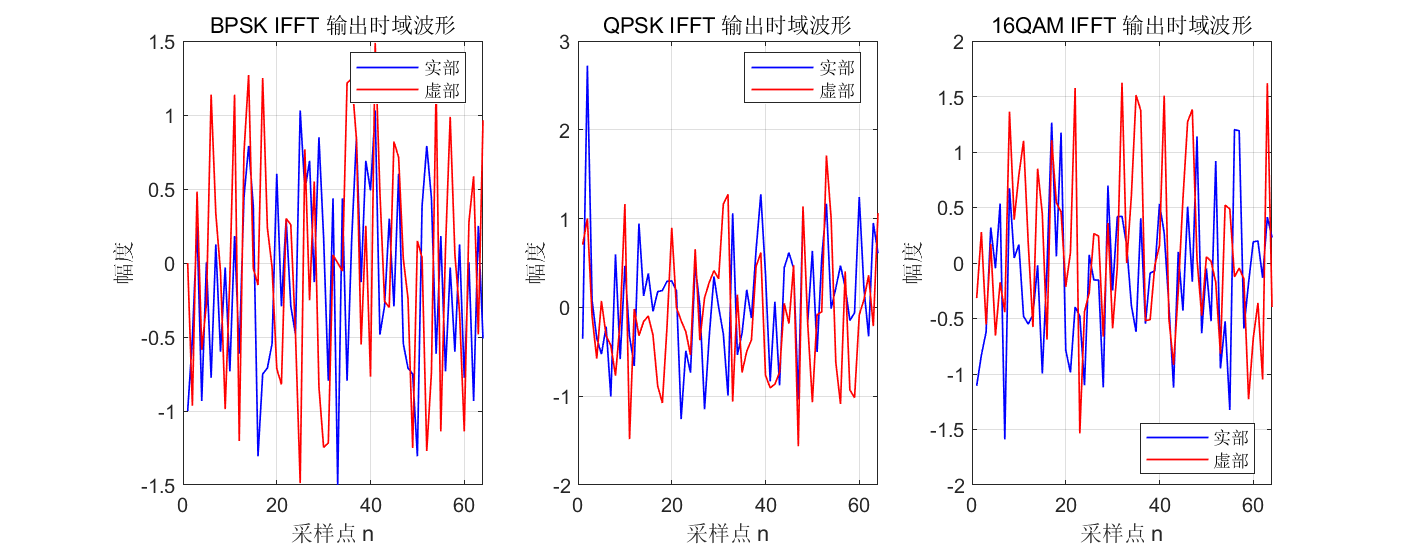
\includegraphics[width=1.0\textwidth]{hw2_step2_ifft.png}
    \caption{三种调制模式下 IFFT 输出的时域基带波形}
    \label{fig:step2_ifft}
\end{figure}

观察图 \ref{fig:step2_ifft}，三种调制模式经 IFFT 后都产生了随机起伏的时域波形。IFFT 的本质是将 $N$ 个不同频率的复正弦波按权重叠加，各子载波的相位随机组合，所以时域波形呈现不规则的包络。BPSK 的子载波只取实数值 $\pm 1$，所以虚部几乎为零；QPSK 和 16-QAM 的子载波取复数值，实部和虚部都有明显的波动。另外可以看到在某些采样点处波形出现较大的峰值，这是多个子载波同相叠加的结果，也是 OFDM 系统峰均功率比偏高的原因之一。

%---------------------------------------------------------------------------------------------------------------------------------
\subsubsection{环节三：AWGN 信道结果与分析}

时域 OFDM 符号 $s(n)$ 经 AWGN 信道传输后，叠加均值为零的复高斯白噪声，得到接收信号 $r(n)$。接收端通过 FFT 将信号还原至频域，得到含噪频域符号 $Y(k)$。

\begin{lstlisting}[caption={环节三：AWGN 信道叠加与 FFT 接收代码}]
% AWGN 信道：叠加高斯白噪声
r_n = awgn(s_n, SNR_dB, 'measured');

% FFT：将接收时域信号变换回频域
Y_k_matrix = (1/sqrt(N_fft)) * fft(r_n, N_fft);
Y_k = Y_k_matrix(:);  % 并串转换
\end{lstlisting}

\begin{figure}[H]
    \centering
    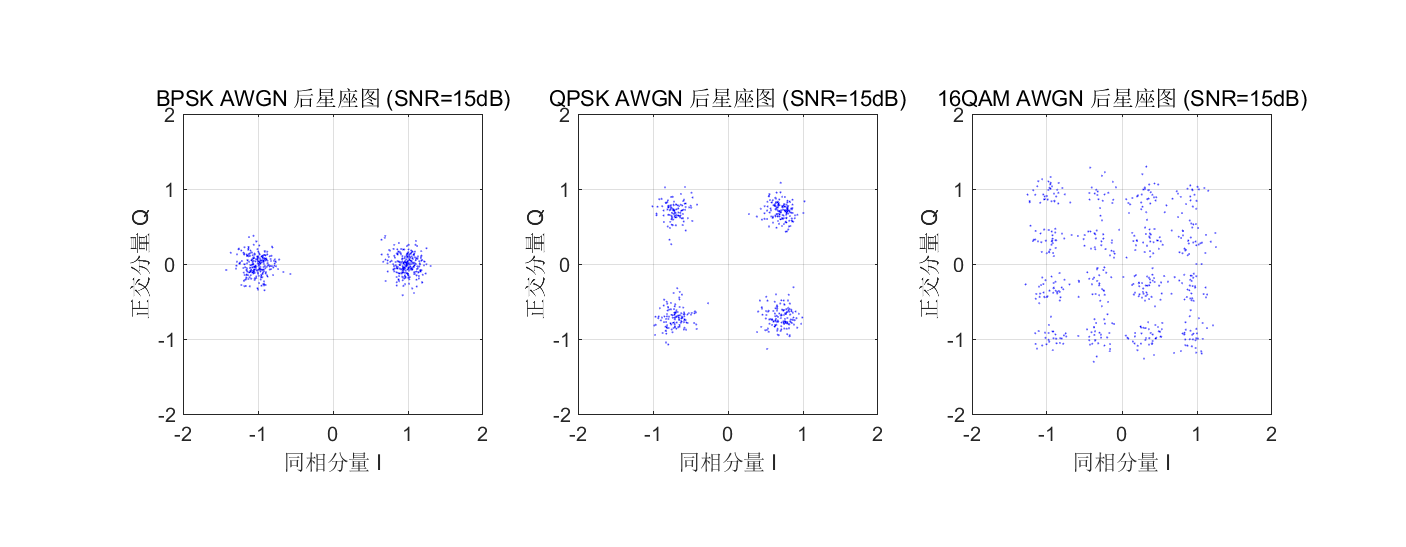
\includegraphics[width=1.0\textwidth]{hw2_step3_awgn.png}
    \caption{AWGN 信道传输后 FFT 输出的星座图 (SNR = 15 dB)}
    \label{fig:step3_awgn}
\end{figure}

图 \ref{fig:step3_awgn} 展示了 SNR $= 15$ dB 条件下三种调制模式经 FFT 恢复后的频域星座图。BPSK 的星座点聚集在 $\pm 1$ 附近，散布范围小；QPSK 的四个簇仍可辨识，但噪声导致的散布已经可见；16-QAM 的 16 个簇散布最为明显，部分点已经接近相邻簇的边界。这说明在相同信噪比下，高阶调制因为星座点间距更小而更容易出现判决错误。

%---------------------------------------------------------------------------------------------------------------------------------
\subsubsection{环节四：FFT 变换结果与分析}

接收端对含噪时域信号 $r(n)$ 执行 $N$ 点 FFT，利用正交性将各子载波信号无损分离，恢复出频域符号 $Y(k)$，随后进行并串转换。

\begin{lstlisting}[caption={环节四：FFT 接收与并串转换代码}]
% FFT：将接收时域信号变换回频域
Y_k_matrix = (1/sqrt(N_fft)) * fft(r_n, N_fft);

% 并串转换：将矩阵展平为串行符号流
Y_k = Y_k_matrix(:);
\end{lstlisting}

\begin{figure}[H]
    \centering
    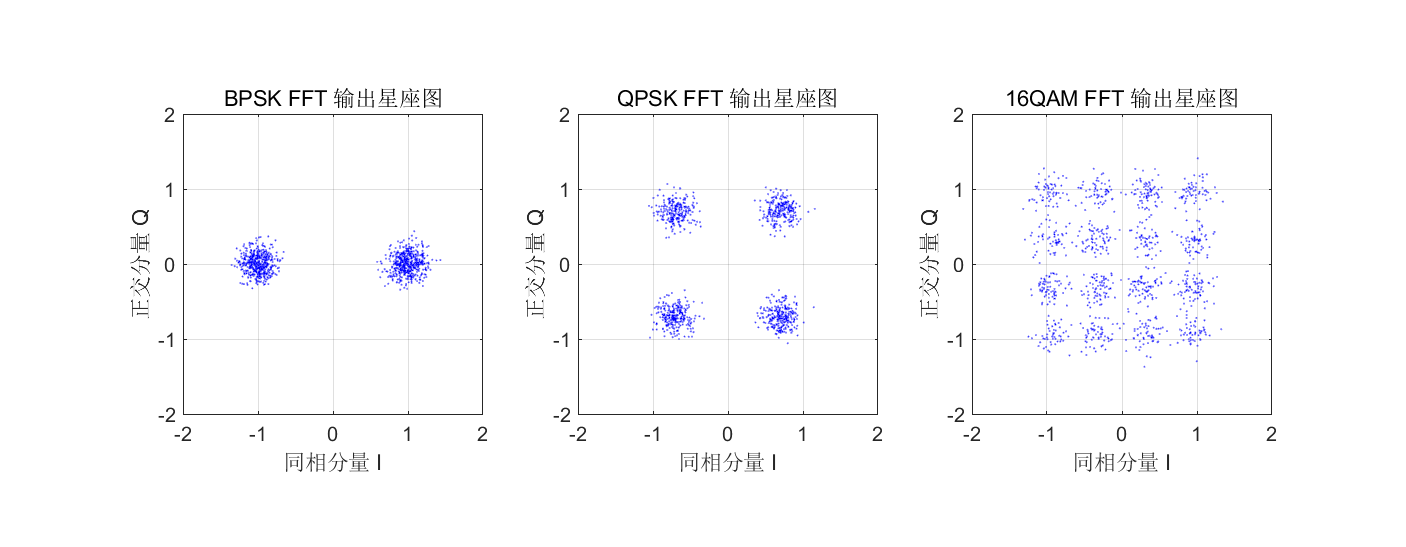
\includegraphics[width=1.0\textwidth]{hw2_step4_fft.png}
    \caption{FFT 输出的频域星座图 (SNR = 15 dB)}
    \label{fig:step4_fft}
\end{figure}

图 \ref{fig:step4_fft} 展示了 FFT 恢复后的频域星座图。由于 FFT 是线性变换，时域高斯白噪声经 FFT 后在频域仍然是独立的高斯噪声，各子载波上的星座点围绕理想位置呈圆形散布。BPSK 的两个簇间距最大，噪声影响很小；QPSK 的四个簇仍然清晰可分；16-QAM 的 16 个簇因为间距小，部分星座点已经进入相邻判决区域。这也说明 FFT 本身不引入失真，误码性能完全取决于调制方式和信道噪声。

%---------------------------------------------------------------------------------------------------------------------------------
\subsubsection{环节五：信号解调结果与分析}

对 FFT 输出的含噪频域符号 $Y(k)$ 依据最小欧氏距离准则进行最大似然判决，将其映射回最近的星座点并逆向恢复为二进制比特流。

\begin{lstlisting}[caption={环节五：最大似然判决与比特恢复代码}]
% 解调判决：最小欧氏距离
if M == 2
    rx_sym = pskdemod(Y_k, M);
    rx_bits = rx_sym;  % BPSK: symbol 0/1 = bit 0/1
else
    rx_bits = qamdemod(Y_k, M, 'OutputType', 'bit', ...
                       'UnitAveragePower', true);
end

% 误码率计算
BER = sum(tx_bits ~= rx_bits) / length(tx_bits);
\end{lstlisting}

\begin{figure}[H]
    \centering
    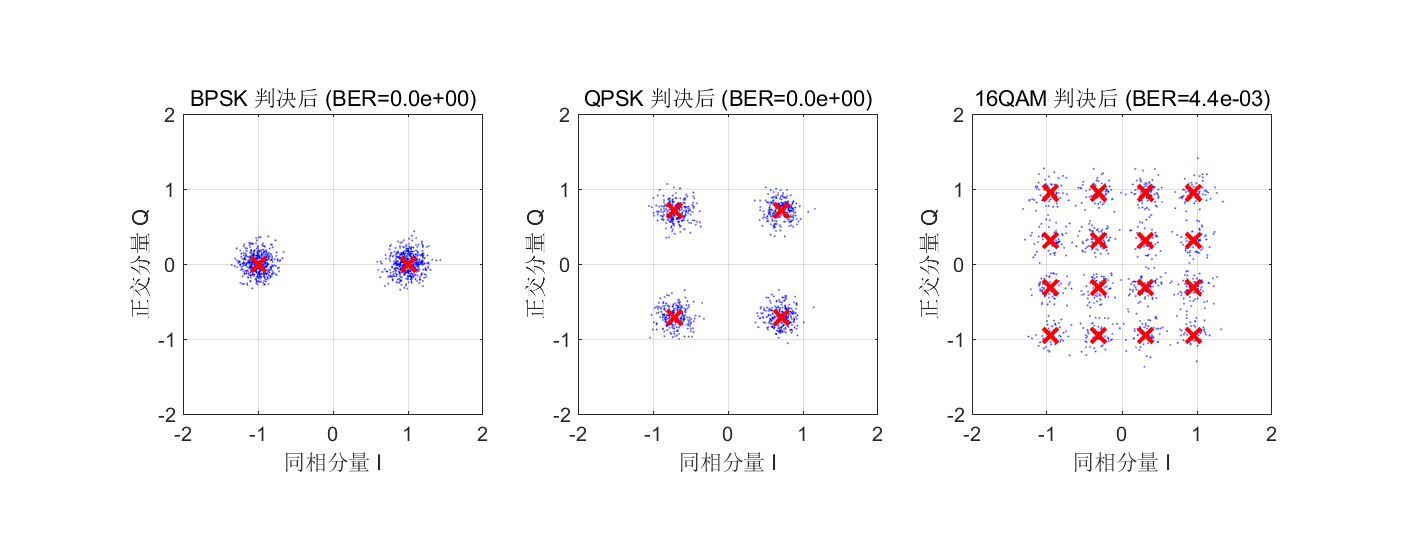
\includegraphics[width=1.0\textwidth]{hw2_step5_demod.png}
    \caption{解调判决后的星座图与误码率（红色叉号为理想星座点）}
    \label{fig:step5_demod}
\end{figure}

图 \ref{fig:step5_demod} 展示了判决后的星座图，红色叉号为各调制模式的标准星座点。在 SNR $= 15$ dB 时，BPSK 与 QPSK 均实现了零误码传输（BER $= 0$），所有接收点都被正确判决；16-QAM 的 BER 约为 $4.5 \times 10^{-3}$，部分接收点因噪声偏移超出了正确判决域。这与理论分析一致：BPSK 星座点距离最大，抗噪能力最强；QPSK 点间距稍小但在这个信噪比下仍然足够；16-QAM 点间距最小，在 15 dB 时噪声已经造成了一定的判决错误。

%---------------------------------------------------------------------------------------------------------------------------------
\subsection{BER 性能曲线分析}

为评估 OFDM 链路在不同信噪比下的传输可靠性，在 SNR $= 0 \sim 20$ dB 范围内进行蒙特卡洛仿真。仿真采用 $N_{fft} = 64$ 个子载波、$N_{syms} = 50000$ 个 OFDM 符号。核心逻辑如下：对每种调制方式先生成全部发送符号并完成 IFFT，然后在外层循环中仅重新叠加不同功率的 AWGN 噪声，这样可以在保证统计独立性的同时大幅节省计算量。

\begin{lstlisting}[caption={蒙特卡洛 BER 仿真核心代码}]
SNR_range = 0:2:20;
ber_sim = zeros(3, length(SNR_range));

for i = 1:3                     % 遍历 BPSK/QPSK/16QAM
    M = M_values(i);
    numBits = N_fft * N_syms * log2(M);
    tx_bits = randi([0 1], numBits, 1);

    % 一次性完成 Mod + S/P + IFFT
    X_k = qammod(tx_bits, M, 'InputType', 'bit', ...
                 'UnitAveragePower', true);
    s_n = sqrt(N_fft) * ifft(reshape(X_k, N_fft, N_syms));

    for j = 1:length(SNR_range) % 外层 SNR 循环
        r_n = awgn(s_n, SNR_range(j), 'measured');
        Y_k = (1/sqrt(N_fft)) * fft(r_n);
        Y_k_serial = Y_k(:);

        rx_bits = qamdemod(Y_k_serial, M, 'OutputType', 'bit', ...
                           'UnitAveragePower', true);
        ber_sim(i,j) = sum(tx_bits ~= rx_bits) / numBits;
    end
end

% 理论曲线：将 Es/N0 转换为 Eb/N0 后调用 berawgn
k = log2(M);
EbNo_range = SNR_range - 10*log10(k);
ber_theory = berawgn(EbNo_range, 'qam', M);
\end{lstlisting}

\begin{figure}[H]
    \centering
    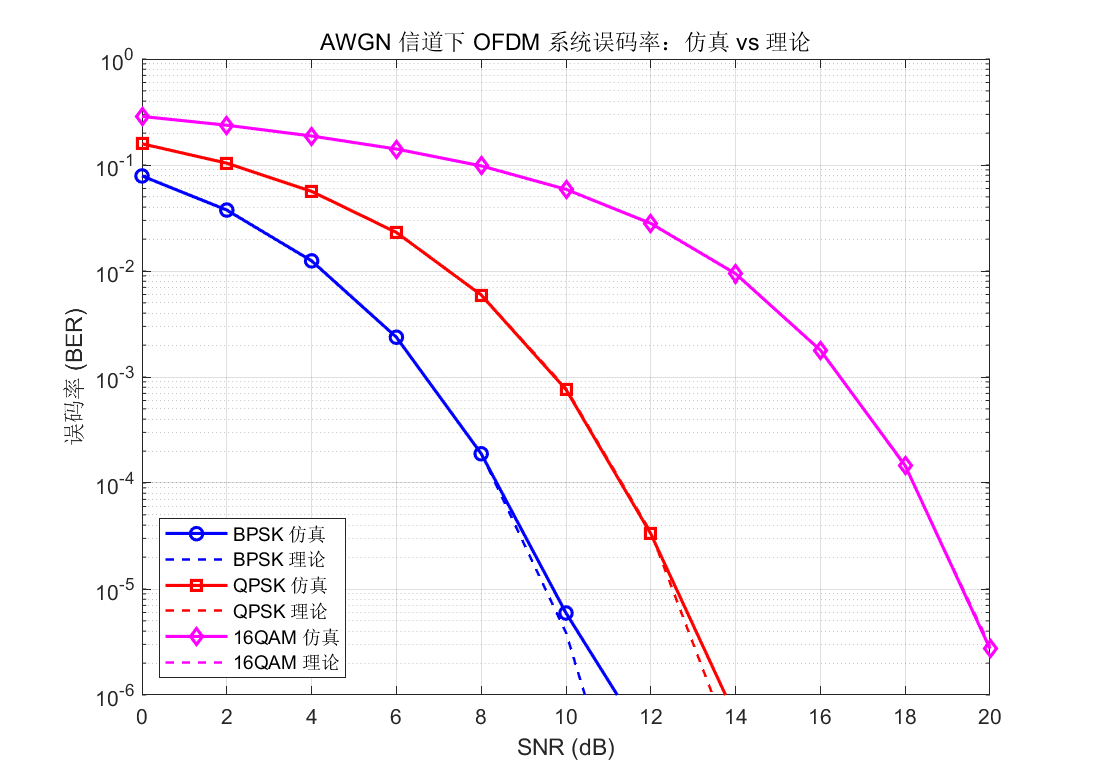
\includegraphics[width=0.75\textwidth]{ber_snr_curve.png}
    \caption{AWGN 信道下 BPSK/QPSK/16-QAM 的 BER：仿真与理论对比}
    \label{fig:ber_curve}
\end{figure}

图 \ref{fig:ber_curve} 中实线为蒙特卡洛仿真结果，虚线为 MATLAB \texttt{berawgn} 函数给出的理论值。可以看到，三种调制方式的仿真点与理论曲线高度吻合，验证了仿真链路的正确性。

为了给出更精确的数据，表 \ref{tab:hw2_ber} 列出了仿真中各调制方式在关键 SNR 节点下的 BER 值。

\begin{table}[H]
\centering
\caption{AWGN 信道下各调制方式的仿真 BER}
\label{tab:hw2_ber}
\begin{tabular}{cccc}
\toprule
SNR (dB) & BPSK & QPSK & 16-QAM \\
\midrule
0  & $7.88 \times 10^{-2}$ & $1.59 \times 10^{-1}$ & $2.87 \times 10^{-1}$ \\
4  & $1.25 \times 10^{-2}$ & $5.64 \times 10^{-2}$ & $1.88 \times 10^{-1}$ \\
8  & $1.89 \times 10^{-4}$ & $5.94 \times 10^{-3}$ & $9.81 \times 10^{-2}$ \\
10 & $5.94 \times 10^{-6}$ & $7.62 \times 10^{-4}$ & $5.90 \times 10^{-2}$ \\
14 & $<10^{-6}$ & $6.25 \times 10^{-7}$ & $9.43 \times 10^{-3}$ \\
18 & $<10^{-6}$ & $<10^{-6}$ & $1.46 \times 10^{-4}$ \\
20 & $<10^{-6}$ & $<10^{-6}$ & $2.73 \times 10^{-6}$ \\
\bottomrule
\end{tabular}
\end{table}

从表 \ref{tab:hw2_ber} 可以看出：
\begin{itemize}
    \item \textbf{BPSK} 在 SNR $= 10$ dB 时 BER 已经低于 $10^{-5}$，在 14 dB 时仿真中已经没有错误比特。
    \item \textbf{QPSK} 在 14 dB 时 BER 约 $6.3 \times 10^{-7}$，与 BPSK 相比性能差距很小，但每符号传输 2 比特。
    \item \textbf{16-QAM} 在 20 dB 时 BER 为 $2.7 \times 10^{-6}$，相比 BPSK/QPSK 恶化了约 6 dB，这是用频谱效率换抗噪声能力的代价。
\end{itemize}


%---------------------------------------------------------------------------------------------------------------------------------
\section{基于 CP 与频域均衡的完整 OFDM 系统仿真}

\subsection{本章引言}

前两章分别完成了多径信道特性分析和 AWGN 信道下的 OFDM 链路仿真。但在实际多径信道中，时延扩展会导致 OFDM 符号之间产生符号间干扰，同时破坏子载波间的正交性。本章在发射端引入循环前缀，并在接收端采用迫零频域均衡，构建完整的多径信道 OFDM 系统。

\subsection{系统数学建模}

\subsubsection{1. 循环前缀 (Add CP)}

发射端将 IFFT 输出时域符号 $s(n)$ 的末尾 $N_{CP}$ 个采样点复制并附加至符号头部，形成带 CP 的发送信号：
\begin{equation}
    s_{CP}(n) = \begin{cases} s(n + N - N_{CP}), & 0 \le n < N_{CP} \\ s(n - N_{CP}), & N_{CP} \le n < N_{CP} + N \end{cases}
\end{equation}
其中 $N_{CP}$ 为 CP 长度，需满足 $N_{CP} \ge L - 1$（$L$ 为信道抽头数），以确保多径时延被 CP 完全吸收。

\subsubsection{2. 多径信道滤波}

带 CP 的信号经多径信道 $h(n) = [h_0, h_1, \dots, h_{L-1}]$ 传输，这是一个线性卷积过程。由于 CP 的存在，去除 CP 后的有效 OFDM 符号与信道之间等效为循环卷积，因此频域关系为逐点相乘：
\begin{equation}
    Y(k) = H(k) \cdot X(k) + W(k)
\end{equation}
其中 $H(k) = \text{DFT}\{h(n)\}$ 为信道的离散频率响应，$W(k)$ 为频域噪声分量。

\subsubsection{3. 去除 CP (Remove CP)}

接收端截取信号的后 $N$ 个采样点，去除循环前缀，恢复标准长度的 OFDM 符号。

\subsubsection{4. ZF 频域均衡}

对 FFT 输出的频域符号执行迫零均衡，即除以信道频率响应 $H(k)$：
\begin{equation}
    \hat{X}(k) = \frac{Y(k)}{H(k)} = X(k) + \frac{W(k)}{H(k)}
\end{equation}
ZF 均衡可以消除信道引入的幅度和相位失真，但在 $H(k)$ 较小的深衰落子载波处，噪声会被放大。

\subsection{仿真参数配置}

本仿真采用如下系统参数：

\begin{table}[H]
\centering
\begin{tabular}{ll}
\toprule
参数 & 取值 \\
\midrule
子载波数 $N$ & 64 \\
OFDM 符号数 & 50000 \\
CP 长度 $N_{CP}$ & 16 \\
信道 $h(n)$ & $[1, 0, 0, 0.5, 0, 0, 0.3, 0, 0.1]$ \\
信道长度 $L$ & 9 \\
\bottomrule
\end{tabular}
\caption{OFDM 系统仿真参数}
\end{table}

关于 CP 长度的选取：信道长度 $L = 9$，因此 CP 只需 $\ge 8$ 即可消除 ISI。本仿真选取 $N_{CP} = 16$，即 $N_{fft}/4 = 64/4 = 16$。在实际通信标准（如 LTE、WiFi）中，CP 长度通常设为 IFFT 点数的 1/4（常规 CP）或 1/2（扩展 CP），这是频谱效率与信道防护之间的工程折中：CP 越长保护越强，但传输效率越低（本例中 CP 开销为 $16/(64+16) = 20\%$）。

此外，第三章 AWGN 仿真中使用的单点信噪比为 $\text{SNR} = 15$ dB。本章为了更清晰地展示多径信道对信号的影响，将单点演示信噪比调整为 $\text{SNR} = 20$ dB，代码中显式重新赋值：

\begin{lstlisting}[caption={本章 SNR 参数设置}]
SNR_dB = 20;  % 本章单点演示信噪比（高于 HW2 的 15 dB）
\end{lstlisting}

\subsection{信道频率响应分析}

\begin{lstlisting}[caption={多径信道冲激响应与频域响应计算代码}]
% 多径信道冲激响应
h = [1, 0, 0, 0.5, 0, 0, 0.3, 0, 0.1];

% 计算 N 点 DFT 得到频域响应
H_k = fft(h, N_fft);
\end{lstlisting}

\begin{figure}[H]
    \centering
    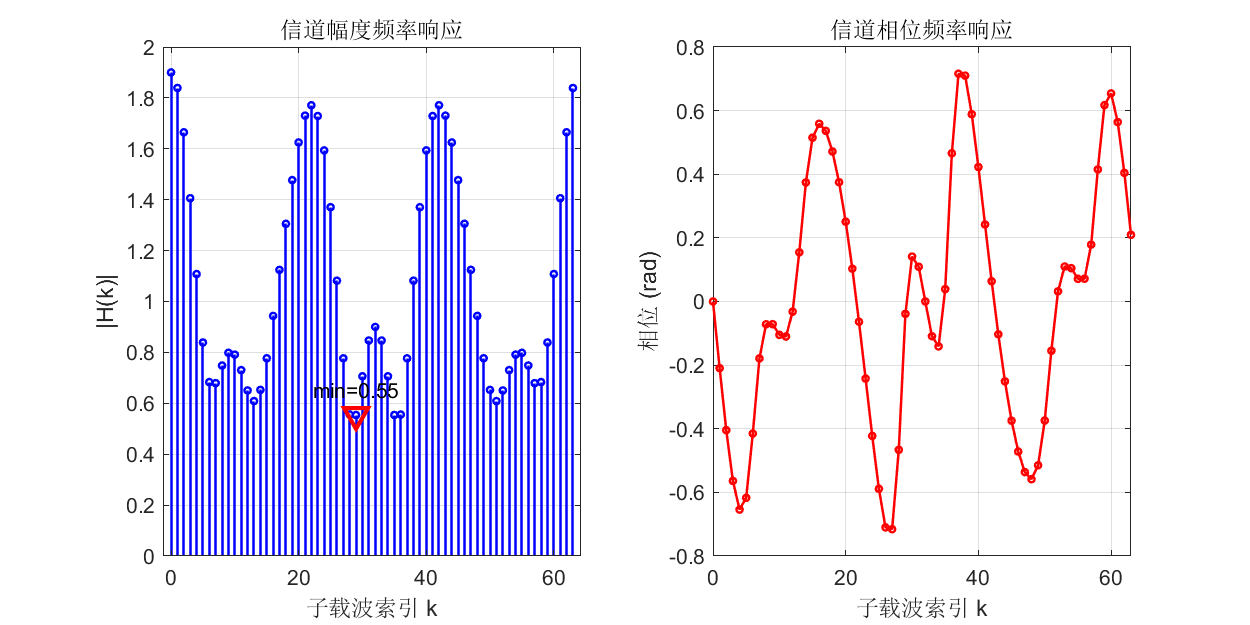
\includegraphics[width=0.9\textwidth]{hw3_channel_Hk.png}
    \caption{多径信道的幅度与相位频率响应}
    \label{fig:hw3_Hk}
\end{figure}

图 \ref{fig:hw3_Hk} 展示了信道的频率响应。幅度响应存在明显的不规则起伏，其中最深的衰落出现在子载波 $k=29$ 处，$|H(29)| = 0.554$，对应深衰落频点。该频点处的噪声放大倍数为：
\begin{equation}
    \frac{\sigma_{eq}^2}{\sigma^2} = \frac{1}{|H(29)|^2} = \frac{1}{0.554^2} = 3.26 \quad (\text{即 } 5.1 \text{ dB})
\end{equation}
这意味着在 $k=29$ 处，ZF 均衡后的等效噪声功率是平均值的 3.26 倍，该子载波的 BER 将明显高于其他子载波。这是 ZF 均衡的核心缺陷：深衰落处噪声被放大。

\subsection{OFDM 链路各环节仿真}

\subsubsection{环节一：信号调制}

\begin{lstlisting}[caption={发射端调制代码}]
numBits = N_fft * N_syms * log2(M);
tx_bits = randi([0 1], numBits, 1);
X_k = qammod(tx_bits, M, 'InputType', 'bit', 'UnitAveragePower', true);
\end{lstlisting}

系统生成随机二进制比特流，经 16-QAM 调制映射为复数符号序列 $X(k)$，并施加单位平均功率归一化。

\subsubsection{环节二：IFFT 变换}

\begin{lstlisting}[caption={串并转换与 IFFT 代码}]
X_k_matrix = reshape(X_k, N_fft, N_syms);
s_n = sqrt(N_fft) * ifft(X_k_matrix, N_fft);
\end{lstlisting}

串行符号经串并转换后重塑为 $N \times N_{syms}$ 矩阵，再逐列执行 IFFT，将频域符号调制到 $N$ 个正交子载波上，合成为时域 OFDM 符号。

\subsubsection{环节三：添加循环前缀 (Add CP)}

\begin{lstlisting}[caption={循环前缀添加代码}]
% 复制每个 OFDM 符号末尾 CP_len 个采样点至头部
s_cp = [s_n(N_fft-CP_len+1:end, :); s_n];
\end{lstlisting}

将每个 OFDM 符号末尾 $N_{CP} = 16$ 个采样点复制到头部。CP 的作用有两个：一是吸收多径时延，消除 ISI；二是将线性卷积转为循环卷积，使频域均衡成为可能。

\subsubsection{环节四：多径信道滤波与频域响应计算}

\begin{lstlisting}[caption={多径信道滤波代码（连续数据流）}]
% 多径信道冲激响应
h = [1, 0, 0, 0.5, 0, 0, 0.3, 0, 0.1];

% 将带 CP 的矩阵展平为一维连续数据流
s_cp_vec = s_cp(:);

% 对连续流做线性卷积（保留符号间 ISI）
r_cp_vec = filter(h, 1, s_cp_vec);

% 恢复矩阵形式
r_cp = reshape(r_cp_vec, size(s_cp));

% 叠加 AWGN
r_cp = awgn(r_cp, SNR_dB, 'measured');
\end{lstlisting}

这里有一个关键点：多径信道滤波必须将所有 OFDM 符号展平为一维连续数据流后再送入 \texttt{filter}，而不是逐符号独立滤波。这是因为实际无线电波是连续传播的，前一个符号尾部的多径时延会泄漏到后一个符号的头部，形成符号间干扰。如果逐列独立滤波，\texttt{filter} 会在每列开始时重置内部状态，等于人为消除了 ISI，使得 CP 失去意义。展平后滤波保留了物理真实的 ISI，而 CP 的作用正是吸收这部分泄漏。

\subsubsection{环节五：去除 CP 与 FFT 接收}

\begin{lstlisting}[caption={去除 CP 与 FFT 代码}]
% 去除循环前缀
r_n = r_cp(CP_len+1:end, :);

% FFT 变换回频域
Y_k_matrix = (1/sqrt(N_fft)) * fft(r_n, N_fft);
\end{lstlisting}

接收端截除每个符号的前 $N_{CP}$ 个采样点，然后执行 FFT 恢复频域符号。此时频域接收符号满足 $Y(k) = H(k) \cdot X(k) + W(k)$。

\subsubsection{环节六：ZF 频域均衡}

\begin{lstlisting}[caption={迫零频域均衡代码}]
% ZF 均衡：除以信道频率响应
Y_k_eq_matrix = Y_k_matrix ./ repmat(H_k(:), 1, N_syms);
\end{lstlisting}

对 FFT 输出逐子载波除以 $H(k)$，完成迫零均衡。均衡后信道的幅度和相位失真被消除，但深衰落子载波处的噪声会被放大。

\subsubsection{环节七：信号解调与误码率}

\begin{lstlisting}[caption={解调判决与 BER 计算代码}]
% 并串转换
Y_k_serial = Y_k_eq_matrix(:);

% 最大似然判决
rx_bits = qamdemod(Y_k_serial, M, 'OutputType', 'bit', ...
                   'UnitAveragePower', true);

% 误码率计算
BER = sum(tx_bits ~= rx_bits) / length(tx_bits);
\end{lstlisting}

均衡后的符号经并串转换和最大似然判决恢复为二进制比特流。

\subsection{均衡效果对比分析}

\begin{figure}[H]
    \centering
    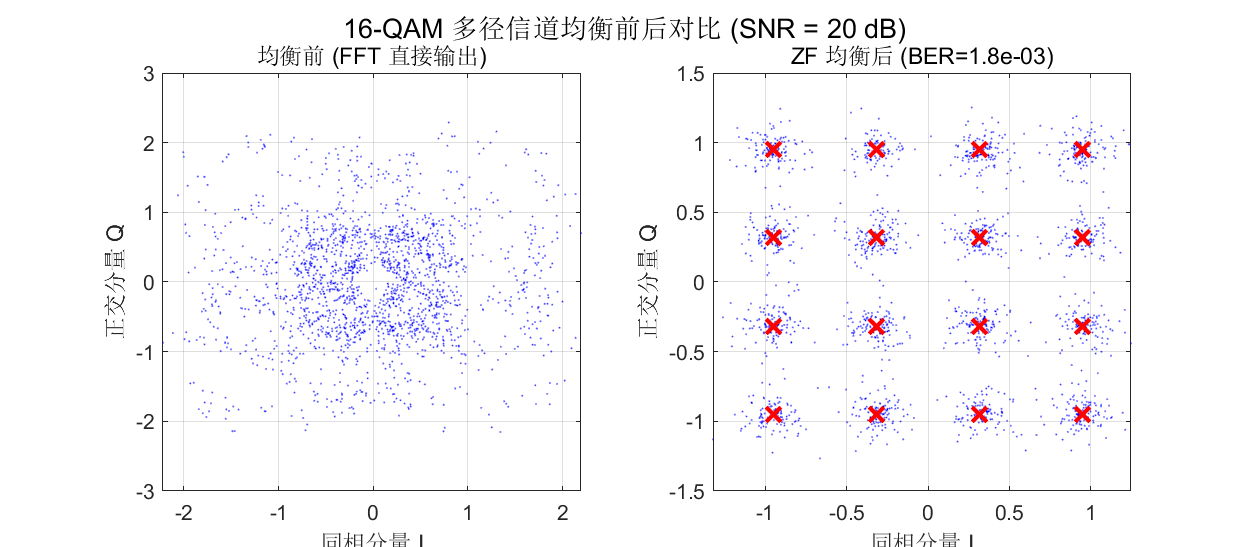
\includegraphics[width=1.0\textwidth]{hw3_equalization_compare.png}
    \caption{16-QAM 多径信道下均衡前后的星座图对比 (SNR = 20 dB)}
    \label{fig:hw3_eq_compare}
\end{figure}

\subsubsection{频率选择性衰落效果分析}

对比图 \ref{fig:hw3_Hk} 的信道频率响应和图 \ref{fig:hw3_eq_compare} 左图（均衡前星座图），可以看出多径信道对信号的影响。均衡前的星座点严重散布，没有形成规则的簇。这是因为多径信道的频率选择性衰落使得不同子载波经历了不同的幅度衰减和相位旋转：深衰落频点处的信号被大幅衰减，对应的星座点靠近原点；而其他频点可能衰减较小甚至增强。这种不均匀的衰落导致星座图上同时出现了散布大和散布小的区域。

\subsubsection{均衡效果分析}

对比图 \ref{fig:hw3_eq_compare} 左右两图，ZF 均衡的效果很明显。均衡后星座点紧密聚集在理想星座点（红色叉号）周围，恢复为规则的高斯散布，说明信道造成的幅度和相位失真已经被补偿。

不过残余的噪声散布并不是完全均匀的。由前面分析可知，$k=29$ 处 $|H(29)| = 0.554$，ZF 均衡后该子载波的等效噪声功率放大了 $1/0.554^2 = 3.26$ 倍（5.1 dB），因此深衰落子载波对应的星座点散布会比其他子载波更大。这也是 ZF 均衡相比 MMSE 均衡的主要缺陷。

整体 BER 为 $1.74 \times 10^{-3}$，明显高于 AWGN 信道下的 $2.73 \times 10^{-6}$，说明 ZF 均衡虽然消除了信道失真，但噪声放大效应导致了性能损失。

\subsubsection{发射与接收比特流对比}

仿真统计得到 16-QAM 在 SNR $= 20$ dB 时的 BER 为 $1.74 \times 10^{-3}$，对应约 1280 万个传输比特中有约 22274 个错误比特。对比发送和接收比特流，绝大部分比特一致，说明 CP + ZF 均衡方案在多径信道下确实能够消除 ISI。但 ZF 均衡的噪声放大效应使得 BER 明显高于同等 SNR 下的 AWGN 信道。

\subsection{多径信道下 BER 性能曲线}

为全面评估系统在多径信道下的传输可靠性，本节在 SNR $= 0 \sim 24$ dB 范围内对三种调制模式进行蒙特卡洛仿真。与 AWGN 仿真的区别在于：信道滤波只需在 SNR 循环外执行一次（因为多径信道是固定的 LTI 系统），内层循环仅重新叠加不同功率的噪声，然后依次完成去 CP、FFT、ZF 均衡和解调。核心代码如下：

\begin{lstlisting}[caption={多径信道蒙特卡洛 BER 仿真核心代码}]
SNR_range = 0:2:24;
ber_sim = zeros(3, length(SNR_range));

for i = 1:3                       % 遍历 BPSK/QPSK/16QAM
    M = M_values(i);
    numBits = N_fft * N_syms * log2(M);
    tx_bits = randi([0 1], numBits, 1);

    % 一次性完成 Mod + S/P + IFFT + Add CP
    X_k = qammod(tx_bits, M, 'InputType', 'bit', ...
                 'UnitAveragePower', true);
    s_n = sqrt(N_fft) * ifft(reshape(X_k, N_fft, N_syms));
    s_cp = [s_n(N_fft-CP_len+1:end, :); s_n];

    % 信道滤波也只需做一次（LTI 信道固定）
    s_cp_vec = s_cp(:);
    r_cp_vec = filter(h, 1, s_cp_vec);
    r_cp = reshape(r_cp_vec, size(s_cp));

    for j = 1:length(SNR_range)   % 外层 SNR 循环
        % 仅重新叠加噪声
        r_noisy = awgn(r_cp, SNR_range(j), 'measured');
        % 去 CP
        r_n = r_noisy(CP_len+1:end, :);
        % FFT 回频域
        Y_k_matrix = (1/sqrt(N_fft)) * fft(r_n, N_fft);
        % ZF 频域均衡
        Y_k_eq = Y_k_matrix ./ repmat(H_k(:), 1, N_syms);
        % 并串 + 解调 + 计 BER
        Y_k_serial = Y_k_eq(:);
        rx_bits = qamdemod(Y_k_serial, M, 'OutputType', ...
                           'bit', 'UnitAveragePower', true);
        errors = sum(tx_bits ~= rx_bits);
        if errors == 0
            ber_sim(i,j) = 1 / numBits;
        else
            ber_sim(i,j) = errors / numBits;
        end
    end
end

% AWGN 理论参考（Eb/N0 转换）
k = log2(M);
EbNo_range = SNR_range - 10*log10(k);
ber_awgn = berawgn(EbNo_range, 'qam', M);
\end{lstlisting}

注意代码结构与 AWGN 仿真的两点区别：一是调制和 IFFT 之后多了 Add CP 和信道滤波两个步骤，且信道滤波采用连续流方式以保留符号间 ISI；二是 FFT 之后增加了 ZF 均衡环节。这两步是多径信道仿真相较于纯 AWGN 仿真的核心增量。

图中实线为多径信道仿真结果，虚线为 AWGN 理论参考曲线。

\begin{figure}[H]
    \centering
    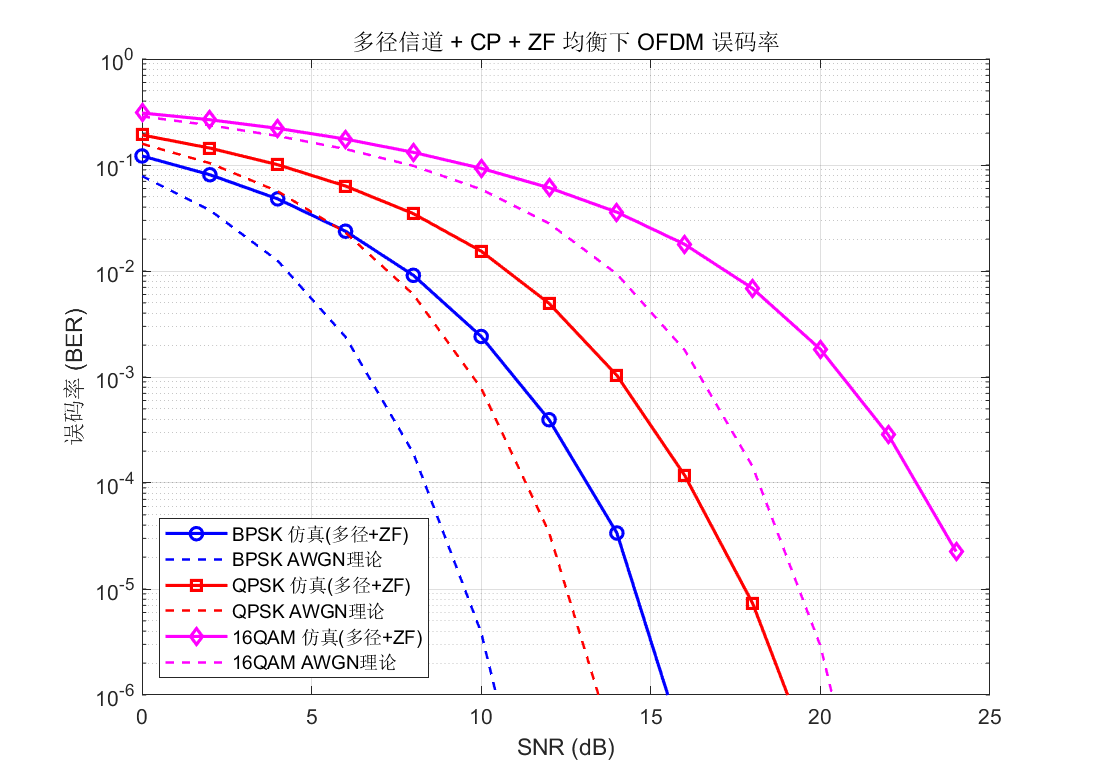
\includegraphics[width=0.75\textwidth]{hw3_ber_curve.png}
    \caption{多径信道 + CP + ZF 均衡下 BER 曲线（实线）vs AWGN 理论（虚线）}
    \label{fig:hw3_ber}
\end{figure}

为便于定量分析，表 \ref{tab:hw3_ber} 列出了关键 SNR 节点下的仿真 BER 值。

\begin{table}[H]
\centering
\caption{多径信道 + ZF 均衡下各调制方式的仿真 BER}
\label{tab:hw3_ber}
\begin{tabular}{cccc}
\toprule
SNR (dB) & BPSK & QPSK & 16-QAM \\
\midrule
0  & $1.21 \times 10^{-1}$ & $1.91 \times 10^{-1}$ & $3.08 \times 10^{-1}$ \\
4  & $4.71 \times 10^{-2}$ & $9.95 \times 10^{-2}$ & $2.20 \times 10^{-1}$ \\
8  & $8.82 \times 10^{-3}$ & $3.41 \times 10^{-2}$ & $1.30 \times 10^{-1}$ \\
10 & $2.31 \times 10^{-3}$ & $1.50 \times 10^{-2}$ & $9.21 \times 10^{-2}$ \\
14 & $2.97 \times 10^{-5}$ & $9.83 \times 10^{-4}$ & $3.53 \times 10^{-2}$ \\
16 & $<10^{-6}$ & $1.08 \times 10^{-4}$ & $1.74 \times 10^{-2}$ \\
20 & $<10^{-6}$ & $1.56 \times 10^{-7}$ & $1.75 \times 10^{-3}$ \\
24 & $<10^{-6}$ & $<10^{-7}$ & $2.09 \times 10^{-5}$ \\
\bottomrule
\end{tabular}
\end{table}

从图 \ref{fig:hw3_ber} 和表 \ref{tab:hw3_ber} 可以得出以下结论：

\begin{itemize}
    \item 三条仿真曲线均高于对应的 AWGN 理论曲线，这是 ZF 均衡在深衰落子载波处放大噪声的代价。以 16-QAM 为例，达到 $\text{BER} = 10^{-3}$ 在 AWGN 信道下仅需约 14 dB，但多径信道下需要约 20 dB，损失了约 6 dB。
    \item BPSK 和 QPSK 在 SNR $= 16$ dB 时已经接近零误码，鲁棒性较好。
    \item 16-QAM 在 24 dB 时 BER 仍有 $2.09 \times 10^{-5}$，距离 AWGN 理论值差距最大，说明高阶调制对 ZF 噪声放大更加敏感。
    \item 想要进一步提升性能，可以考虑将 ZF 均衡替换为 MMSE 均衡（$\hat{X}(k) = H^*(k) Y(k) / (|H(k)|^2 + \sigma^2)$），在深衰落处通过引入偏差来抑制噪声放大。
\end{itemize}

%---------------------------------------------------------------------------------------------------------------------------------
\section{总结}

本报告通过三个递进的仿真实验，系统地研究了 OFDM 数字通信系统的核心原理。

第一部分通过建立双径和多径离散信道模型，分别研究了第二径时延、幅度、相位以及多径数量对信道频率响应的影响。仿真结果验证了时延扩展与相干带宽的反比关系，以及幅度接近时会产生深衰落、相位变化只会平移衰落位置等基本规律。

第二部分搭建了基于 IFFT/FFT 的 OFDM 基带链路，在 AWGN 信道下对比了 BPSK、QPSK 和 16-QAM 三种调制方式。通过逐步展示调制、IFFT、加噪、FFT、解调五个环节的信号变化，直观呈现了 OFDM 的工作过程。BER 曲线表明，BPSK 和 QPSK 性能接近，16-QAM 在高频谱效率的同时需要更高的信噪比。

第三部分在系统中加入了循环前缀和迫零频域均衡，在多径信道环境下完成了完整的 OFDM 传输仿真。均衡前后的星座图对比清楚地展示了频率选择性衰落的影响以及 ZF 均衡的补偿效果。BER 曲线进一步表明，多径信道下 ZF 均衡会放大深衰落处的噪声，高阶调制对此更加敏感。

通过本次实验，我对 OFDM 系统中多径信道、循环前缀、频域均衡等关键技术的原理和作用有了更深入的理解。


\end{document}